\documentclass[a4paper,12pt]{article}
\usepackage[a4paper, portrait, margin=0.5in]{geometry}
\usepackage[utf8]{inputenc}
\usepackage[spanish]{babel}
\selectlanguage{spanish}
\usepackage{amsmath}
\usepackage{amsfonts}
\usepackage{polynomial}
\usepackage{makeidx}
\usepackage{graphicx}
\usepackage{lmodern}

\begin{document}
\newcommand{\osf}[2]{\dfrac{#1^2}{#2^2}}
\newcommand{\T}{\Big(2\pi\cdot\sqrt{\dfrac{l}{g}}\Big)}
\newcommand{\alpa}{\dfrac{e^{x \beta -3}{2y\beta +5}}}
\newcommand{\deriv}[2]{\dfrac{\delta #1}{\delta #2}}
\newcommand{\sderiv}[3]{\dfrac{\delta ^2 #1}{\delta #2 \delta #3}}
\newcommand{\ext}{e^{ax-bt}}
\newcommand{\exy}{e^{((x-1)^2 + (y-3)^2}}
\newcommand{\xo}{\vec{x_0}} %Devuelve un vector x_0

\begin{titlepage}
	\centering
	{\scshape\LARGE Universidad Autónoma de México \par}
	\vspace{1cm}
	{\scshape\Large Matemáticas para las Ciencias Aplicadas III\par}
	\vspace{1.5cm}
	{\huge\bfseries Tarea I\par}
	\vspace{.5cm}
	{\Large\itshape Alan Ernesto Arteaga Vázquez \par}
    \vspace{.5cm}
	{\Large\itshape Alma Rocío Sánchez Salgado \par}
    \vspace{.5cm}
	{\Large\itshape Jerónimo Almeida Rodríguez \par}
	\vfill
	 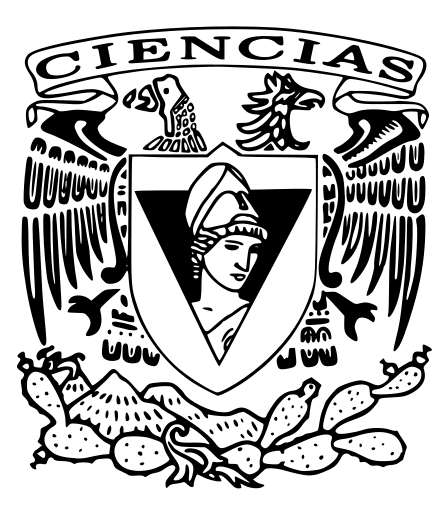
\includegraphics[width=0.5\textwidth]{../escudo_f-ciencias.png}
	\vfill

% Bottom of the page
	{\large Jueves 23 de Agosto del 2018 \par}
\end{titlepage}

\newpage

\section{Marsden - Tromba | Sección 3.3}

\textit{18. Sea $f(x,y,z) = x^2 + y^2 + z^2 + kyz$}
\begin{itemize}
	\item[a] Comprobar que $(0,0,0)$ es punto crítico para $f$.
	$$\nabla f = \langle \deriv{f}{x}, \deriv{f}{y}, \deriv{f}{z}\rangle = \langle 2x, 2y + kz, 2z +ky \rangle$$
	Igualando las parciales a $0$, tenemos que
	\begin{itemize}
		\item[i] Si $2x = 0$, entonces $x = 0$.
	s	\item[ii] Si $2y + kz = 0$, entonces $2y = -kz$ y $y = \dfrac{-kz}{2}$.
		\item[iii] Si $2z + ky = 0$, entonces $z = \dfrac{-ky}{2}$ y por (ii) $z = \dfrac{-k (\dfrac{-kz}{2})}{2} = \dfrac{k^2z}{4}$.
	\end{itemize}
	Además, por (iii) tenemos que $z = \dfrac{k^2z}{4} \Rightarrow \dfrac{z}{z} = \dfrac{k^2}{4} \Rightarrow 1 = \dfrac{k^2}{4} \\ \Rightarrow 4 = k^2 \Rightarrow k = \pm 2$\\
	De (ii) y de (iii) podemos ver que para que se cumpla la igualdad, $y = 0$ y $z = 0$.\\
	Por lo tanto, $f(x,y,z)$ tiene un punto crítico en  $(0,0,0)$.
	\item[b] Cómo $k$ es una constante y el punto crítico de la función es cuándo $x = y = z = 0$, entonces $k \in (-\infty, \infty)$ porque por propiedades de campo, sabemos que $kyz = k(0) = 0$.\\
	Por lo tanto, $k$ puede tomar cualquier valor.\\
\end{itemize}
\textit 34. Sea $f(x,y) = 5ye^x - e^{5x} -y^5$
\begin{itemize}
	\item[a] Demuestre que  $f$ tiene un único punto crítico que también es máximo de $f$.
	Para encontrar el punto crítico hacemos $\nabla f = 0$. Así,
	\begin{itemize}
		\item[i] $\deriv{f}{x} = 5ye^x-5e^{5x}$. Entonces, $\deriv{f}{x} = 0$ cuando $5ye^x-5e^{5x} = 0$.
		\item[ii]$\deriv{f}{y} = 5e^x-5y^4$. Entonces, $\deriv{f}{y} = 0$ cuando $5e^x-5y^4 = 0$.
	\end{itemize}
	De (i) tenemos entonces que $5e^x = 5e^{5x} \Rightarrow ye^x = e^5x$\\
	De (ii) tenemos que $5e^x = 5y^4 \Rightarrow e^x = y^4$ De esta ecuación, proponemos al vector $\xo = (0,1)$.\\
	Evaluando (ii) en $\xo$ tenemos que
	$$ e^x = e^0 = 1 = 1^4 = y^4$$
	Y, evaluando (i) en $\xo$ tenemos que
	$$ye^x = 1\cdot e^0 = e^0 = 1 = e^{5\cdot 0} = e^{5x}$$
	Por lo tanto, $f(\xo)$ es un punto crítico.
	Para comprobar que $\xo$ es máximo, lo evaluamos en el Hessiano.
	\[
	\begin{bmatrix}
	x & y
	\end{bmatrix}
	\begin{bmatrix}
	    \sderiv{f}{x}{x} & \sderiv{f}{x}{y}\\
		\sderiv{f}{y}{x} & \sderiv{f}{y}{y}\\
	\end{bmatrix}
	\begin{bmatrix}
	x \\ y
	\end{bmatrix}\\
	=
	\begin{bmatrix}
	x & y
	\end{bmatrix}
	\begin{bmatrix}
	    5ye^x - 25e^{5x} & 5e^x\\
		5e^x & -20y^3\\
	\end{bmatrix}
	\begin{bmatrix}
	x \\ y
	\end{bmatrix}\\
	=
	\]
	\[
	\begin{bmatrix}
	x & y
	\end{bmatrix}
	\begin{bmatrix}
	    5ye^x - 25e^{5x} & 5e^x\\
		5e^x & -20y^3\\
	\end{bmatrix}
	\begin{bmatrix}
	x \\ y
	\end{bmatrix}\\
	=
	\begin{bmatrix}
	x & y
	\end{bmatrix}
	\begin{bmatrix}
	    5(1)e^0 - 25e^{5(0)} & 5e^(0)\\
		5e^(0) & -20(1)^3\\
	\end{bmatrix}
	\begin{bmatrix}
	x \\ y
	\end{bmatrix}\\
	=
	\]
	\[
	\begin{bmatrix}
	x & y
	\end{bmatrix}
	\begin{bmatrix}
	    -20 & 5\\
		5 & -20\\
	\end{bmatrix}
	\begin{bmatrix}
	x \\ y
	\end{bmatrix}\\
	=
	\begin{bmatrix}
	-20x + 5y & 5x - 20y
	\end{bmatrix}
	\begin{bmatrix}
	x \\ y
	\end{bmatrix}\\
	=
	\begin{bmatrix}
	-20x^2+5xy+5xy-20y^2
	\end{bmatrix}
	\]
	Entonces, Hess($\xo$) = $[-20x^2+5xy+5xy-20y^2]|_{\xo} = -20(0)+10(0)(1)-20(1) = -20$\\
	Cómo el Hess($\xo$) $< 0$, entonces $\xo$ es un máximo.
	\item[b] Muestre que $f$ no está acotado en el eje $y$ y por lo tanto no tiene máximo global.
	Fijamos a $x = 0$ y evaluamos la funcion $f(0,y)= 5ye^0-e^0-y^5 = 5y-1-y^5$ y observamos que \[ \lim_{x \to \pm \infty} f(0,y) = \pm \infty \]\\
	Por lo tanto, $f(0,y)$ no está acotada y no tiene máximo global.

\end{itemize}

\textit{23. An examination of the function}
	$$f:\mathbb{R}^2 \mapsto \mathbb{R}, (x, y) \mapsto (y -3x^2)(y -x^2)$$
	\textit{will give an idea of the difficulty of finding conditions that
			guarantee that a critical point is a relative extremum when Theorem
			6 fails. Show that}\\

	\textit{a) the origin is a critical point of $f$ ;}\\

	Procedemos a derivar parcialmente la función, así, se sigue:
	$$f(x,y) = y^2 -3x^2y -x^2y + 3x^4 = y^2 -4x^2y + 3x^4  $$
	$$\frac{\partial f}{\partial x} = -8xy + 12x^3 $$
	$$\frac{\partial f}{\partial y} = 2y - 4x^2 $$

	luego, para ver que precisamente el origen es un punto crítico,
	evaluamos las parciales en dicho punto, así:
	$$\left. \frac{\partial f}{\partial x} \right|_{(0,0)}
			= -8(0)(0) + 12(0)^3 = 0 $$
	$$\left. \frac{\partial f}{\partial y} \right|_{(0,0)}
			= 2(0) - 4(0)^2 = 0 $$

	así, como todas las parciales son cero en el origen, se sigue que este es
	un punto crítico.\\

	\textit{b) $f$ has a relative minimum at $(0, 0)$ on every straight line
			through $(0, 0)$; that is, if $g(t) = (at, bt)$, then
			$f \circ g : \mathbb{R} \rightarrow \mathbb{R}$ has a relative
			minimum at 0,for every choice of a and b;}\\

		Consideremos ahora a la funcíón $f \circ g$:
		$$ f \circ g = (bt)^2 - 4(at)^2(bt) + 3(at)^4$$
		$$ = b^2t^2 - 4a^2bt^3 + 3a^4t^4$$

		ahora, derivando la función compuesta, se tiene:
		$$\frac{\partial f}{\partial t} = 2b^2t -12a^2bt^2 + 12a^4t^3
										= 2t(b^2 - 6a^2bt + 6a^4t^2)$$

		se sigue que $t = 0$ es un punto crítico correspondiente a $(x,y) = (0,0)$.
		Ahora, derivando nuevamente la función, se tiene:

		$$\frac{\partial^2 f}{\partial t^2} = 2b^2 -24a^2bt + 36a^4t^2 $$

		ahora, evaluando la segunda derivada en el punto $t = 0$
		$$\left. \frac{\partial^2 f}{\partial t^2} \right|_{0}
			= 2b^2 -24a^2b(0) + 36a^4(0)^2 = 2b^2 $$

		como
			$$\left. \frac{\partial^2 f}{\partial t^2} \right|_{0} = 2b^2 > 0$$
		se sigue que $t = 0$ es un mínimo local para
		$\forall a$ si $b \neq 0$\\

		Ahora, si $b = 0$, se cumple que
			$$f \circ g (t) = 3(at)^4$$
		así que $t = 0$ resulta ser un mínimo local para cualquier elección de
		$a$ y $b$.\\

	\textit{(c) the origin is not a relative minimum of $f$ .}\\
	\newline

	\textit{\textbf{$27.$}Suppose $f: \mathbb{R}^3 \mapsto \mathbb{R}$ is $C^2$, and that $x_{0}$ is a critical point for $f$. Suppose $Hf (x_{0})(h) = h_{1}^2 + h_{2}^2 + h_{3}^2 + 4h_{2}h_{3}$ Does $f$ have a local maximum, minimum, or saddle a $x_{0}$?}\
\textit{\textbf{51.}
	\begin{itemize}
		\item[(a)] Let f be a $C^1$ function on the real line $\mathbb{R}$. Suppose that f has exactly one critical point $x_{0}$ that is a strict local minimum for $f$ . Show that $x_{0}4$ is also an absolute minimum for $f$; that is, that $f(x) \geq f(x_{0})$ for all $x$.
		\item[(b)] The next example shows that the conclusion of part (a) does not hold for functions of more tha one variable. Let $f: \mathbb{R}^2 \mapsto \mathbb{R}$ be defined by
		\[f(x,y) = -y^4-e^{-x^2}+2y^2 \sqrt{e^x + e^{-x^2}}\]
	\end{itemize}
}


	\textit{41. Find the absolute maximum and minimum values for
		$$f(x, y) = sin x + cos y$$ on the rectangle $R$ defined by
		$$0 \leq x \leq 2\pi, 0 \leq y \leq 2\pi$$}

		Derivando parcialmente, se tiene:
		$$\frac{\partial f}{\partial x} = \cos x $$
		$$\frac{\partial f}{\partial y} = - \sin x $$

		ahora, para los intervalos $0 \leq x \leq 2\pi, 0 \leq y \leq 2\pi$
		se cumple:
			$$\frac{\partial f}{\partial x} = 0 \quad \text{si} \quad
				x=\frac{\pi}{2}, \frac{3\pi}{2}$$
			$$\frac{\partial f}{\partial y} = 0 \quad \text{si} \quad
				y=0, \pi, 2\pi$$

		así, se sigue que la función tiene puntos críticos en:
			$$(\frac{\pi}{2}, 0), (\frac{\pi}{2}, \pi), (\frac{\pi}{2}, 2\pi)$$
			$$(\frac{3\pi}{2}, 0), (\frac{3\pi}{2}, \pi), (\frac{3\pi}{2}, 2\pi)$$

		ahora, construimos la matriz Hessiana para la función derivando
		parcialmente por segunda vez a la función, así:
			$$ \frac{\partial^2f}{\partial x^2} = -\sin x$$
			$$ \frac{\partial^2f}{\partial x\partial y} = 0 = \frac{\partial^2f}{\partial y\partial x}$$
			$$ \frac{\partial^2f}{\partial y^2} = - \cos y$$

			$$H(x,y) = \begin{bmatrix}
    					\dfrac{\partial^2f}{\partial x^2} & & \dfrac{\partial^2f}{\partial x\partial y} \\
    					& & \\
    					\dfrac{\partial^2f}{\partial y\partial x}&  & \dfrac{\partial^2f}{\partial y^2} \\
						\end{bmatrix} =
						\begin{bmatrix}
			    			-\sin x & 0 \\
			    			0  & - \cos y \\
						\end{bmatrix}
						$$

		luego, evaluando la matriz en los puntos críticos y sacando su determinante,
		se tiene:
		$$det[H(\frac{\pi}{2}, 0)] =
			\begin{vmatrix}
				-\sin \dfrac{\pi}{2} & 0 \\
				0  & - \cos 0 \\
			\end{vmatrix} =
			\begin{vmatrix}
				-1 & 0 \\
				 0 & -1 \\
			\end{vmatrix} = 1$$

		Como $f_{xx} < 0$ y $det(H) > 0$, entonces corresponde a un máximo local.\\
		$$det[H(\frac{\pi}{2}, \pi)] =
			\begin{vmatrix}
				-\sin \dfrac{\pi}{2} & 0 \\
				0  & - \cos \pi \\
			\end{vmatrix} =
			\begin{vmatrix}
				-1 & 0 \\
				 0 & 1 \\
			\end{vmatrix} = -1$$
		Como $f_{xx} < 0$ y $det(H) < 0$, entonces corresponde a un punto de ensilladura.\\
		$$det[H(\frac{\pi}{2}, 2\pi)] =
			\begin{vmatrix}
				-\sin \dfrac{\pi}{2} & 0 \\
				0  & - \cos 2\pi \\
			\end{vmatrix} =
			\begin{vmatrix}
				-1 & 0 \\
				 0 & -1 \\
			\end{vmatrix} = 1$$
		Como $f_{xx} < 0$ y $det(H) > 0$, entonces corresponde a un máximo local.\\


		$$det[H(\frac{3\pi}{2}, 0)] =
			\begin{vmatrix}
				-\sin \dfrac{3\pi}{2} & 0 \\
				0  & - \cos 0 \\
			\end{vmatrix} =
			\begin{vmatrix}
				1 & 0 \\
				 0 & -1 \\
			\end{vmatrix} = -1$$

		Como $f_{xx} > 0$ y $det(H) < 0$, entonces corresponde a un punto de ensilladura.\\
		$$det[H(\frac{3\pi}{2}, \pi)] =
			\begin{vmatrix}
				-\sin \dfrac{3\pi}{2} & 0 \\
				0  & - \cos \pi \\
			\end{vmatrix} =
			\begin{vmatrix}
				1 & 0 \\
				 0 & 1 \\
			\end{vmatrix} = 1$$
		Como $f_{xx} > 0$ y $det(H) > 0$, entonces corresponde a un mínimo local.\\
		$$det[H(\frac{3\pi}{2}, 2\pi)] =
			\begin{vmatrix}
				-\sin \dfrac{3\pi}{2} & 0 \\
				0  & - \cos 2\pi \\
			\end{vmatrix} =
			\begin{vmatrix}
				1 & 0 \\
				 0 & -1 \\
			\end{vmatrix} = -1$$
		Como $f_{xx} > 0$ y $det(H) < 0$, entonces corresponde a un punto de ensilladura.\\


		Luego, evaluando máximos locales en la función para determinar
		máximos absolutos:
			$$ f(\frac{\pi}{2}, 0) = \sen(\frac{\pi}{2}) + cos(\pi) = 1 + 1 = 2 $$
			$$ f(\frac{\pi}{2}, 2\pi) = \sen(\frac{\pi}{2}) + cos(2\pi) = 1 + 1 = 2$$

		así, determinamos que la función $f$ tiene máximos absolutos en los puntos
			$$(\frac{\pi}{2}, 0), (\frac{\pi}{2}, 2\pi)$$
		y mínimo absoluto en
			$$(\frac{3\pi}{2}, \pi)$$

	\section{Marsden - Tromba | Sección 3.4}
	\textit{\textbf{26.}An irrigation canal in Arizona has concrete sides and bottom with trapezoidal cross section of area
 $A = y(x + y \tan \theta)$ and wetted perimeter \\
 $P = x + \dfrac{2y}{\cos \theta}$, where $x = $bottom width, $y = $water depth, and $\theta =$side inclination, measured
 from vertical.The best design for a fixed inclination $\theta$ is found by solving $P =$ minimum subject to the condition
 $A =$ constant. Show that $y^2 =\dfrac{A \cos \theta}{2 - \sin \theta}$
}
	\section{Hughes-Hallet | Sección 16.1}
	\textit{\textbf{5.} Figure $16.8$ shows a contour plot of population density, people per square kilometer, in a rectangle of land $3$ km by $2$ km. Estimate the population in the refion represented by Figure $16.8$}

Sea R el rectángulo y $f(x,y)$ la densidad poblacional en el punto $(x,y)$, la población está dada por $\int_{R}f(x,y)dA$.. Si aproximamos la integral con sumas de Riemann usando la información de cada km por km, entonces podemos tomar la densidad en un un punto y sumarlos.
Vamos a dividir el eje $y$ en dos partes y el eje $x$ en tres, tenemos los puntos:
(0.5, 1.5)=500, (0.5, 0.5)= 650, (1.5,1.5)= 450, (1.5, 0.5)=200, (2.5, 1.5)=100 y (2.5, 0.5)= 400
por lo que la densidad por km cuadrado es la suma de estos valores
\[\int_{R}(x,y)dA\approx 500 + 450 + 100 + 650 + 200 + 400 = 2300\]

\textit{\textbf{6-12} Decide(without calculation) wheter the integrals are positive, negative, or zero. Let $D$ be the region inside the unit circle centered at the origin, let $R$ be the rigth half of $D$ and let $B$ be the bottom half of $D$}
\begin{itemize}
	\item[6.]$\int_{D}dA$
	         Es positiva, la integral de $f(x,y) = 1$
	\item[7.]$\int_{R}5xdA$
			  La integral es positiva, tomemos en cuenta que es la mitad derecha del área total del círculo unitario, entonces toma x toma valores mayores a $0$. La función siendo integrada es $f(x,y) = 5x$
	\item[8.]$\int_{B}5xdA$
			  B es una función simétrica respecto a $x$ por lo que la integral se cancela: $f(x,y) = -f (-x,y)$ y el resutado es cero.
	\item[9.]$\int_{D}(y^3 + y^5)dA$
		  	   D es simétrico respecto a $y$, por lo que la integral es cero también
	\item[10.]$\int_{B}(y^3+y^5)dA$
			   Los valores de la función con $y < 0$ (porque es la mitad de abajo del círculo)son negativos,por lo que la integral también lo es.
	\item[11.]$\int_{D}(y-y^3)dA$
				$f(x,y) = y- y^3$ es una función impar, y D es simétrica respecto a $y$ por lo que la integral se cancela y es igual a cero
	\item[12.]$\int_{B}(y-y^3)dA$
			 La función $f(x,y) = y -y^3$ es negativa en la región B ya que todos los valores de $y$ en esa región son negativos, entonces tenemos que $\mid y^3 \mid < \mid y \mid$ por lo que la integral es negativa.
\end{itemize}
	\section{Anton-Bivens-Davis | Sección 14.1}
	\textit{\textbf{10.} $\int^{\pi}_{\pi / 2}\int^2_1 x \cos xy dy dx$}\
En nuestra herramienta de cálculo pusimos :
N[Integrate[x Cos[x y], {x, 1, 2}, {y, Pi/2, Pi}]] y nos arroja :
\[int^{\pi}_{\pi /2}\int^2_1 x \cos xy dy dx = - \dfrac{4}{\pi} \approx -1.27324\]

	\textit{\textbf{18.} (a) Let $f(x,y) = x - 2y$,and as shown in Exercise 17,
	let the rectangle $ R = [0, 2] x [0, 2]$ be subdivided into 16 subrectangles.\\
	\newline
	Take $(x^{*}_{k}, y^{*}_{k})$ to be the center of the $k-th$ rectangle, and approximate
	the double integral of f over R by the resulting Riemann sum.}\\

	Se tiene, que como $(x^{*}_{k}, y^{*}_{k})$ corresponden a los puntos medios
	de cada uno de los $k$ rectángulos, es necesario calcular el valor de cada
	uno de los puntos bajo la función $f$, así, como el rectángulo R está
	comprendido entre

		$$ 0 \leq x \leq 2, 0 \leq y \leq 2  $$

	y dicho rectángulo se divide en 16 rectángulos de igual tamaño, se sigue que
	los puntos medios de todos los rectángulos corresponden a los puntos:

		$$ (\frac{1}{4}, \frac{7}{4}), (\frac{3}{4}, \frac{7}{4}),
			(\frac{5}{4}, \frac{7}{4}), (\frac{7}{4}, \frac{7}{4}) $$
		$$ (\frac{1}{4}, \frac{5}{4}), (\frac{3}{4}, \frac{5}{4}),
			(\frac{5}{4}, \frac{5}{4}), (\frac{7}{4}, \frac{5}{4}) $$
		$$ (\frac{1}{4}, \frac{3}{4}), (\frac{3}{4}, \frac{3}{4}),
			(\frac{5}{4}, \frac{3}{4}), (\frac{7}{4}, \frac{3}{4}) $$
		$$ (\frac{1}{4}, \frac{1}{4}), (\frac{3}{4}, \frac{1}{4}),
			(\frac{5}{4}, \frac{1}{4}), (\frac{7}{4}, \frac{1}{4}) $$

	así, evaluando los puntos bajo la función, se obtiene:

	$$ f(\frac{1}{4}, \frac{7}{4}) =  - \frac{13}{4}, \quad f(\frac{3}{4}, \frac{7}{4}) =  - \frac{11}{4} , \quad
	   f(\frac{5}{4}, \frac{7}{4}) =  - \frac{9}{4} , \quad f(\frac{7}{4}, \frac{7}{4}) = - \frac{7}{4} $$

	$$ f(\frac{1}{4}, \frac{5}{4}) =  - \frac{9}{4}, \quad f(\frac{3}{4}, \frac{5}{4}) =  - \frac{7}{4} , \quad
	   f(\frac{5}{4}, \frac{5}{4}) =  - \frac{5}{4} , \quad f(\frac{7}{4}, \frac{5}{4}) = - \frac{3}{4} $$

	$$ f(\frac{1}{4}, \frac{3}{4}) =  - \frac{5}{4}, \quad f(\frac{3}{4}, \frac{3}{4}) =  - \frac{3}{4} , \quad
	   f(\frac{5}{4}, \frac{3}{4}) =  - \frac{1}{4} , \quad f(\frac{7}{4}, \frac{3}{4}) = \frac{1}{4} $$

	$$ f(\frac{1}{4}, \frac{1}{4}) =  - \frac{1}{4}, \quad f(\frac{3}{4}, \frac{1}{4}) = \frac{1}{4} , \quad
	   f(\frac{5}{4}, \frac{1}{4}) =  \frac{3}{4} , \quad f(\frac{7}{4}, \frac{1}{4}) = \frac{5}{4} $$

	luego, la suma de Riemann resultante está dada por:

	$$ \sum_{k=1}^{16} f(x^{*}_{k}, y^{*}_{k}) \Delta A_{k} = - \frac{1}{4}(1) +
	  	\frac{1}{4}(1) + \frac{3}{4}(1) + \frac{5}{4}(1) + (- \frac{5}{4})(1) +
		(- \frac{3}{4})(1) + (- \frac{1}{4})(1) + \frac{1}{4}(1)  $$
	$$ + (- \frac{9}{4})(1) + (- \frac{7}{4})(1) + (- \frac{5}{4})(1) + (- \frac{3}{4})(1)
	   + (- \frac{13}{4})(1) + (- \frac{11}{4})(1) + (- \frac{9}{4})(1) + (- \frac{7}{4})(1) $$
	$$  = - \frac{1}{4} + \frac{1}{4} + \frac{3}{4} + \frac{5}{4} + - \frac{5}{4}
		- \frac{3}{4} - \frac{1}{4} + \frac{1}{4}
	    - \frac{9}{4} - \frac{7}{4} - \frac{5}{4} - \frac{3}{4}
	    - \frac{13}{4} - \frac{11}{4} - \frac{9}{4} - \frac{7}{4} $$

	$$  = - \frac{9}{4} - \frac{7}{4} - \frac{5}{4} - \frac{3}{4}
	      - \frac{13}{4} - \frac{11}{4} - \frac{9}{4} - \frac{7}{4} $$
	$$ = - \frac{64}{4} = -16 $$

	\textit{ (b) Compare the result in part (a) to the exact value of the integral. }\\

		Ahora, calculando la integral doble para la región delimitada por
		$$ 0 \leq x \leq 2, 0 \leq y \leq 2  $$

		para la función $ f(x,y) = x - 2y $ se tiene:

		$$ \iint\limits_{R} f(x,y)\mathrm{d}A = \int_{0}^{2} \int_{0}^{2} x - 2y \; dx dy  $$
		$$  = \int_{0}^{2} [ \frac{x^2}{2} -2yx] \Big|_0^2 dy $$
		$$  = \int_{0}^{2} \frac{4}{2} -2y(2) \; dy $$
		$$  = \int_{0}^{2} 2 - 4y \; dy $$
		$$  = [ 2y - \frac{4y^2}{2}] \Big|_0^2 $$
		$$  = [ 2y - 2y^2 ] \Big|_0^2 $$
		$$  = 4 - 8  = - 4 $$

		Así, la diferencia ente el resultado en la parte (a) y la parte (b) es de
		$12$ \\
		
	\textit{\textbf{23 - 26 True - False.} Determine whether the statement is
	true or false. Explain your answer.\\}

	\textit{\textbf{23.} In the definition of a double integral}

		$$  \iint\limits_{R} f(x,y)\mathrm{d}A = \lim\limits_{n \rightarrow + \infty}
		 	\sum_{k=1}^{n} f(x^{*}_{k}, y^{*}_{k}) \Delta A_{k} $$

	\textit{ the symbol $ \Delta A_{k}$ represents a rectangular region within $R$
	 		from which the point $ (x^{*}_{k}, y^{*}_{k}) $ is taken.}\\

	Decimos que el enunciado es \textbf{cierto}. Considerememos el siguiente texto extraído
	del libro \textit{Calculus - 10th Edition por Anton /Bivens} para realizar el
	cálculo del volumen entre una superficie $ z = f(x,y)$ y una región $R$, donde
	las secciones resaltadas con negritas sustentan la respuesta: \\

	- Using lines parallel to the coordinate axes, divide the rectangle
	enclosing the region R into subrectangles, and exclude from consideration
	all those subrectangles that contain any points outside of R.
	\textbf{This leaves only rectangles that are subsets of R.} Assume that there are $n$
	such rectangles, and \textbf{denote the area of the kth such rectangle by $A_k$.} \\

	- Choose any arbitrary point in each subrectangle, \textbf{and denote the point in
	the kth subrectangle by $ (x^{*}_{k}, y^{*}_{k}) $.} The product
	$ f(x^{*}_{k}, y^{*}_{k}) \Delta A_k$  is the volume of a rectangular
	parallelepiped with base area $A_k$ and height $f(x^{*}_{k}, y^{*}_{k})$,so the sum

		$$ \sum_{k=1}^{n} f(x^{*}_{k}, y^{*}_{k}) \Delta A_{k} $$

	can be viewed as an approximation to the volume V of the entire solid.\\

	\textit{\textbf{24.} If R is the rectangle $ \{(x,y):1 \leq x \leq 4,0 \leq y \leq 3\} $
			and $\int_{0}^{3} f(x,y) dy = 2x$, then}

		$$ \iint\limits_{R} f(x,y)\mathrm{d}A = 15 $$
	\
	Se tiene que el teorema de Fubini enuncia:\\
	\textit{ Let R be the rectangle defined by the inequalities $a \leq x \leq b$, $c \leq y \leq d$ }.\\
	\textit{ If $f(x, y)$ is continuous on this rectangle, then }

		$$ \iint\limits_{R} f(x,y)\mathrm{d}A = \int_{c}^{d} \int_{a}^{b} f(x,y) dx dy
			= \int_{a}^{b} \int_{c}^{d} f(x,y) dy dx  $$

	Así, aplicando el teorema de Fubini, se sigue:
		$$ \iint\limits_{R} f(x,y)\mathrm{d}A = \int_{1}^{4} \int_{0}^{3} f(x,y) dy dx
		 	= \int_{1}^{4} 2x dx = \frac{2x^2}{2} \Big|_1^4 = x^2 \Big|_1^4 = 16 - 1 = 15 $$

		Así, el enunciado resulta ser \textbf{cierto}.\\

	\textit{\textbf{25.} If R is the rectangle $ \{(x,y):1 \leq x \leq 5,2 \leq y \leq 4\} $,
			then}

		$$ \iint\limits_{R} f(x,y)\mathrm{d}A = \int_{1}^{5} \int_{2}^{4} f(x,y) dx dy $$

	De igual forma, aplicando el teorema de Fubini, como en ele ejercicio anterior se tiene:

		$$ \iint\limits_{R} f(x,y)\mathrm{d}A = \int_{2}^{4} \int_{1}^{5} f(x,y) dx dy $$

			o bien:

		$$ \iint\limits_{R} f(x,y)\mathrm{d}A = \int_{1}^{5} \int_{2}^{4} f(x,y) dy dx $$

	pero la integral propuesta no puede suceder, dados los límites que caractrizan
	al rectángulo $R$ por lo que, se sigue que el enunciado es \textbf{falso}.\\

	\textit{\textbf{26.} Suppose that for some region R in the xy-plane}
			$$ \iint\limits_{R} f(x,y)\mathrm{d}A = 0 $$
	\textit{ If $R$ is subdivided into two regions $R_1$ and $R_2$, then }
			$$ \iint\limits_{R_1} f(x,y)\mathrm{d}A = - \iint\limits_{R_2} f(x,y)\mathrm{d}A  $$

	Citando al libro \textit{Calculus} de Anton-Bivens, en la página 1006, en un
	apartado de Propiedades de Integales Dobles, menciona lo siguiente:\\

	\textit{It is evident intuitively that if $f(x, y)$ is nonnegative on a
	region R, then subdividing R into two regions $R_1$ and $R_2$ has the effect
	of subdividing the solid between R and $z = f (x , y)$ into two solids,
	the sum of whose volumes is the volume of the entire solid. This suggests
	the following result, which holds even if $f$ has negative values:}

		$$ \iint\limits_{R} f(x,y)\mathrm{d}A
			= \iint\limits_{R_1} f(x,y)\mathrm{d}A + \iint\limits_{R_2} f(x,y)\mathrm{d}A  $$

	Ahora, aplicando dicha propiedad al problema, se sigue por hipótesis:

		$$ 0 = \iint\limits_{R} f(x,y)\mathrm{d}A
			= \iint\limits_{R_1} f(x,y)\mathrm{d}A + \iint\limits_{R_2} f(x,y)\mathrm{d}A  $$

	y así :

		$$ 0 = \iint\limits_{R_1} f(x,y)\mathrm{d}A + \iint\limits_{R_2} f(x,y)\mathrm{d}A  $$

	con lo que se sigue, conmutando la igualdad :

		$$ \iint\limits_{R_1} f(x,y)\mathrm{d}A + \iint\limits_{R_2} f(x,y)\mathrm{d}A = 0$$

	y de allí se obtiene :

		$$ \iint\limits_{R_1} f(x,y)\mathrm{d}A = - \iint\limits_{R_2} f(x,y)\mathrm{d}A $$

	Con lo cual, concluimos que el enunciado resulta ser \textbf{cierto}.\\

	\textit{\textbf{28.}Use the result in Exercise 27 to evaluate the integral
	\[\int^{ln 3}_{0} \int^1_-1 \sqrt{e^y + 1}\tan x dx dy\]
	by inspection. Explain your reasoning}\ \\

	\textit{\textbf{33}}\\

	\textit{\textbf{39.} Suppose that the temperature in degrees Celsius at a
	point $(x,y)$ on a flat metal plate is $ T(x,y)=10 - 8x^2 - 2y^2$, where x
	and y are in meters. Find the average temperature of the rectangular portion
	of the plate for which $0 \leq x \leq 1$ and $0 \leq y \leq 2$.}\\

	Se tiene, pues que para calcular la temperatura promedio de un área
	determinada, esta está dada mediante la integral doble :

		$$ \frac{1}{A}  \iint\limits_{R} T(x,y)\mathrm{d}A   $$

	donde A representa al área $ 0 \leq x \leq 1$, $ 0 \leq y \leq 2 $ de la
	placa metálica.\\

	Luego, calculando la integral doble se tiene:

		$$ \iint\limits_{R} T(x,y)\mathrm{d}A  =
			\int_{0}^{2} \int_{0}^{1} 10 - 8x^2 - 2y^2 \mathrm{d}x \mathrm{d}y   $$

		$$ = \int_{0}^{2} [ 10x - \frac{8x^3}{3} - 2xy^2 ] \Big|_0^1 \mathrm{d}y $$
		$$ = \int_{0}^{2} 10 - \frac{8}{3} - 2y^2  \mathrm{d}y $$
		$$ = \int_{0}^{2} \frac{30}{3} - \frac{8}{3} - 2y^2 \mathrm{d}y $$
		$$ = \int_{0}^{2} \frac{22}{3} - 2y^2 \mathrm{d}y $$
		$$ = [ \frac{22}{3}y - \frac{2y^3}{3} ] \Big|_0^2$$
		$$ = \frac{44}{3} - \frac{16}{3} $$
		$$ = \frac{28}{3} $$

	Luego, se tiene que como el área de la placa metálica está comprendida entre
	$ 0 \leq x \leq 1 $ y $ 0 \leq y \leq 2 $, entonces se sigue:

	 	$$ A = (1 - 0) * (2 - 0) = 1 * 2 = 2  $$

	luego, sustituyendo en la fórmula para obtener la temperatura promedio, se
	tiene:
		$$ \frac{1}{A}  \iint\limits_{R} T(x,y)\mathrm{d}A  = \frac{1}{2} (\frac{28}{3}) $$
		$$ = \frac{28}{6} = \frac{14}{6} $$
\end{document}
